%% wp7 补布局、逻辑乘积/逻辑切分、结论与致谢（论文收尾）
\wpsh{补}
\label{sec:complement}

布局（layout）$\v{L} : \Z(\v{L}) \to \D$ 的\emph{补}（complement）是一个满足下列条件的布局 $\v{L}^* : \Z(\v{L}^*) \to \D$
\begin{align}
\label{eqn:comp:congruence}
\text{与陪域弱同余：} && \D \lesssim \v{L}^*, \\
\label{eqn:comp:disjoint}
\text{像互不相交：} && \forall b \in \Z(\v{L}), \ \forall a \in \Z^{\v{L}^*}/\{0\}, \ &\v{L}(b) \neq \v{L}^*(a), \\
\label{eqn:comp:ordered}
\text{像有序：} && \forall a \in \Z_{\abs{\v{L}^*}}/\{0\}, \ &\v{L}^*(a-1) < \v{L}^*(a).
%\text{\emph{???:}} && \v{L}^\dagger (\v{L}, \v{L}^*) \v{L}^\dagger = \v{L}^\dagger
\end{align}
布局的补是一个在原布局的陪域（codomain）之中、但不在其像（image）之中生成元素的布局。在复合（Composition）中，布局 $\v{L}$ 常被用作对另一个布局的间接寻址，因此补 $\v{L}^*$ 就是指向 $\v{L}$ 所遗漏元素的那个布局。{\tt complement} 操作使得可以经由\emph{逻辑切分}（logical divide）（第~\ref{sec:logical_divide}~节）切分布局，并经由\emph{逻辑乘积}（logical product）（第~\ref{sec:logical_product}~节）实现布局的重复与扩展。

本节只关注陪域 $\D$ 为 {\tt HTuple}($\Z$) 的布局：即整数，或对某个轮廓 D 而言 $\D = \Z^D$ 的坐标。这使得弱同余条件式~\eqref{eqn:comp:congruence} 得以成立。像互不相交条件（式~\eqref{eqn:comp:disjoint}）保证补所生成的值与原布局生成的值互不相同。注意，这里使用的是原布局的有限定义域 $\Z(\v{L})$，而使用的是补的无穷扩展定义域 $\Z^{\v{L}^*}$。这保证了无论补的形状被截断还是被扩展（例如通过与右侧的布局复合），它所生成的值始终与原布局不同。最后，像有序条件（式~\eqref{eqn:comp:ordered}）确立了补布局的唯一性。

表~\ref{tab:complements} 给出了补的若干例子。

\begin{table}[ht]
\begin{center}
\begin{tabular}{|>{$}c<{$}|>{$}c<{$}|c|}
\v{L} & \v{L}^* & 备注 \\ \hline \hline
(4,8):(1,4) & 1:32 & 注意 $\forall i \in \Z^+, \v{L}^*(i) > \max_{j \in \Z_\v{L}} \v{L}(j)$。 \\ \hline
(4,8):(8,1) & 1:32 & 输入的顺序无关紧要。 \\ \hline
(4,(4,2)):(4,(1,16)) & 1:32 & 输入的层级结构无关紧要。 \\ \hline
(4,8):(1,5) & 1:40 \\ \hline
(4,8):(1,8) & (2,1):(4,64) & 仍然互不相交，但在陪域中“填补空洞”。 \\ \hline
((2,2),(2,4)):((0,1),(0,2)) & 1:8 & 步幅（stride）为 0 的模无贡献。 \\ \hline
((2,2),(2,4)):((0,2),(0,4)) & (2,1):(1,16) \\ \hline
(4,8):(e_0,e_1) & (1,1):(4e_0,8e_1) & 结果定义域与陪域 $\Z^{(\ast,\ast)}$ 同余。 \\ \hline
(4,(4,2)):(e_1,(e_0,12e_1)) & (1,(3,1)):(4e_0,(4e_1,24e_1)) & 弱同余、互不相交且有序。 \\ \hline
\end{tabular}
\end{center}
\caption{布局补的例子。}
\label{tab:complements}
\end{table}

\wpssh{应用：逻辑乘积}
\label{sec:logical_product}

两个布局 $\v{A}$ 与 $\v{B}$ 的逻辑乘积是一个布局 $\v{R}$，其中“布局 $\v{B}$ 的每个元素都被替换为布局 $\v{A}$ 的一个经过唯一平移的版本”。

具体地，我们将逻辑乘积定义为一个从两个布局产生一个 2 阶（rank-2）布局的函数
\begin{align*}
\v{A} \otimes \v{B} = (\v{A}, \v{A}^* \circ \v{B})
\end{align*}
其中 $\v{A}^*$ 是 $\v{A}$ 的补。注意，结果的第一个模（mode）恰好就是输入布局 $\v{A}$，而第二个模在元素形状（shape）与元素顺序上与输入布局 $\v{B}$ 相容。第一个模，即 $\v{A}$ 布局，通常被称为“瓦片”，它在“网格”布局 $\v{B}$ 上被重复。%Because the purpose of the logical product is to expand the domain and codomain of $\v{A}$, this does not require that $(\v{A},\v{A}^*)$ is surjective onto $\Z_{\norm{\v{B}}}$.

考虑这样的例子：行主序（row-major）布局 $(\textcolor{red}{3},\textcolor{red}{4}):(\textcolor{red}{4},\textcolor{red}{1})$ 瓦片，要在列主序（col-major）布局 $(\textcolor{blue}{2},\textcolor{blue}{5}):(\textcolor{blue}{1},\textcolor{blue}{2})$ 网格中复现：
\begin{align*}
\begin{array}{cc} (\textcolor{red}{3}, & \textcolor{red}{4}) \\ (\textcolor{red}{4}, & \textcolor{red}{1}) \end{array}
\ \otimes \
\begin{array}{cc} (\textcolor{blue}{2}, & \textcolor{blue}{5}) \\ (\textcolor{blue}{1}, & \textcolor{blue}{2}) \end{array}
\ =\
\left(
\begin{array}{cc} (\textcolor{red}{3}, & \textcolor{red}{4}) \\ (\textcolor{red}{4}, & \textcolor{red}{1}) \end{array}, \
\begin{array}{c} 1 \\ 12 \end{array}
\ \circ \
\begin{array}{cc}(\textcolor{blue}{2}, & \textcolor{blue}{5}) \\ (\textcolor{blue}{1},& \textcolor{blue}{2}) \end{array}
\right)
\ = \
\begin{array}{cccc}((\textcolor{red}{3}, & \textcolor{red}{4}), & (\textcolor{blue}{2}, & \textcolor{blue}{5})) \\ ((\textcolor{red}{4}, & \textcolor{red}{1}), & (\textcolor{blue}{12}, & \textcolor{blue}{24})) \end{array}
\end{align*}
其中布局 $1:12$ 是 $(\textcolor{red}{3},\textcolor{red}{4}):(\textcolor{red}{4},\textcolor{red}{1})$ 的补。在结果的第一个模中可以直接得到原始瓦片，而结果的第二个模以 $2\times 5$ 列主序的顺序将原始瓦片不重复地重复 10 次。

作为另一个例子，考虑布局 $(\textcolor{red}{4},\textcolor{red}{8}):(\textcolor{red}{20},\textcolor{red}{2})$ 瓦片在行主序布局 $(\textcolor{blue}{3},\textcolor{blue}{2}):(\textcolor{blue}{2},\textcolor{blue}{1})$ 网格中复现：
\begin{align*}
\begin{array}{cc} (\textcolor{red}{4}, & \textcolor{red}{8}) \\ (\textcolor{red}{20}, & \textcolor{red}{2}) \end{array}
\ \otimes \
\begin{array}{cc} (\textcolor{blue}{3}, & \textcolor{blue}{2}) \\ (\textcolor{blue}{2}, & \textcolor{blue}{1}) \end{array}
\ = \
\left(
\begin{array}{cc} (\textcolor{red}{4}, & \textcolor{red}{8}) \\ (\textcolor{red}{20}, & \textcolor{red}{2}) \end{array}, \
\begin{array}{cc} (2, & 1) \\ (1, & 80) \end{array}
\ \circ \
\begin{array}{cc} (\textcolor{blue}{3}, & \textcolor{blue}{2}) \\ (\textcolor{blue}{2}, & \textcolor{blue}{1}) \end{array}
\right)
\ = \
\begin{array}{cccc}((\textcolor{red}{4}, & \textcolor{red}{8}), & (\textcolor{blue}{3}, & \textcolor{blue}{2})) \\ ((\textcolor{red}{20}, & \textcolor{red}{2}), & (\textcolor{blue}{80}, & \textcolor{blue}{1})) \end{array}
\end{align*}
其中布局 $(2,1):(1,80)$ 是 $(\textcolor{red}{4},\textcolor{red}{8}):(\textcolor{red}{20},\textcolor{red}{2})$ 的补。注意，此时网格在交错排布这些瓦片，以产生结果的最小陪域。补布局告诉结果如何为布局 $\v{B}$ 设定步幅，而布局 $\v{B}$ 告诉结果如何为补布局排序并定形。

\paragraph{相关乘积}

逻辑乘积产生一个 2 阶布局，其中第一个模是原始瓦片，第二个模被解释为该瓦片的网格，即“铺瓦”。

虽然逻辑乘积对 $\v{A}$ 与 $\v{B}$ 的阶（rank）或相容性没有任何限制，但操作 {\tt blocked\_product} 往往是一个更直观的版本，它利用输入的阶来构造结果的形状。我们可能会期望一个 $3 {\times} 4$ 布局与一个 $2 {\times} 5$ 布局的乘积产生一个 $6 {\times} 20$ 布局。{\tt blocked\_product} 要求 $\v{A}$ 与 $\v{B}$ 的阶相同，
\begin{align*}
\text{阶}(\v{A}) = \text{阶}(\v{B})
\end{align*}
以便施加一个 zip 操作，把逻辑上的行模与行模、列模与列模组合起来。例如，将上例中的模重排
\begin{align*}
\begin{array}{cccc}((\textcolor{red}{3}, & \textcolor{red}{4}), & (\textcolor{blue}{2}, & \textcolor{blue}{5})) \\ ((\textcolor{red}{4}, & \textcolor{red}{1}), & (\textcolor{blue}{12}, & \textcolor{blue}{24})) \end{array}
\ \Longrightarrow \
\begin{array}{cccc}((\textcolor{red}{3}, & \textcolor{blue}{2}), & (\textcolor{red}{4}, & \textcolor{blue}{5})) \\ ((\textcolor{red}{4}, & \textcolor{blue}{12}), & (\textcolor{red}{1}, & \textcolor{blue}{24})) \end{array}
\end{align*}
便得到一个 $6 {\times} 20$ 布局。图~\ref{fig:blockedproduct} 画出了得到的布局，其中每个 $3 {\times} 4$ 瓦片都施以底纹。之所以称其为“分块”，是因为结果布局中的每个 $3 {\times} 4$ 块都恰好是原始 $3 {\times} 4$ 瓦片的平移版本。

\begin{figure}[ht]
\centering
%\includegraphics[scale=0.5]{blocked_product}
\scalebox{0.5}{
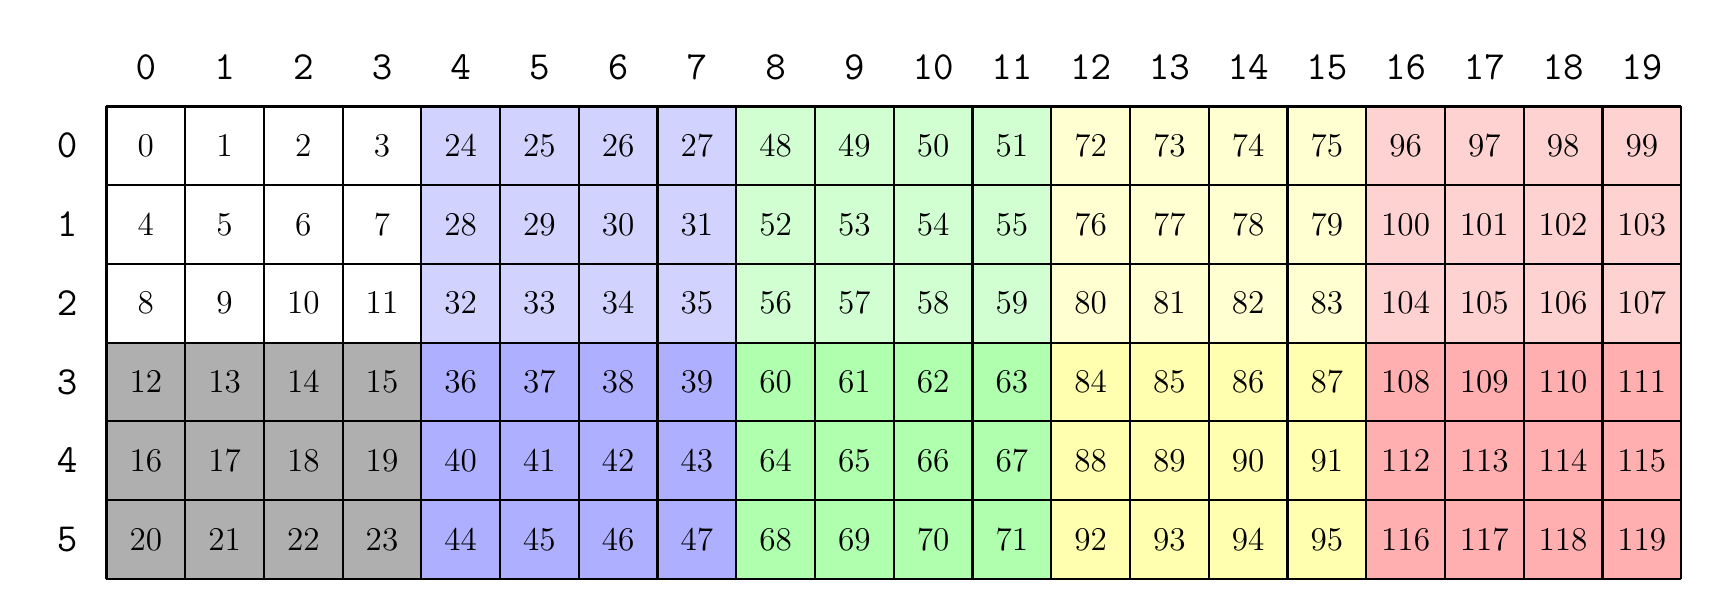
\begin{tikzpicture}[x={(0cm,-1cm)},y={(1cm,0cm)},every node/.style={minimum size=1cm, outer sep=0pt}]
\node[fill={rgb,255:red,255;green,255;blue,255}] at (0,0) {\large 0};
\node[fill={rgb,255:red,255;green,255;blue,255}] at (0,1) {\large 1};
\node[fill={rgb,255:red,255;green,255;blue,255}] at (0,2) {\large 2};
\node[fill={rgb,255:red,255;green,255;blue,255}] at (0,3) {\large 3};
\node[fill={rgb,255:red,210;green,210;blue,255}] at (0,4) {\large 24};
\node[fill={rgb,255:red,210;green,210;blue,255}] at (0,5) {\large 25};
\node[fill={rgb,255:red,210;green,210;blue,255}] at (0,6) {\large 26};
\node[fill={rgb,255:red,210;green,210;blue,255}] at (0,7) {\large 27};
\node[fill={rgb,255:red,210;green,255;blue,210}] at (0,8) {\large 48};
\node[fill={rgb,255:red,210;green,255;blue,210}] at (0,9) {\large 49};
\node[fill={rgb,255:red,210;green,255;blue,210}] at (0,10) {\large 50};
\node[fill={rgb,255:red,210;green,255;blue,210}] at (0,11) {\large 51};
\node[fill={rgb,255:red,255;green,255;blue,210}] at (0,12) {\large 72};
\node[fill={rgb,255:red,255;green,255;blue,210}] at (0,13) {\large 73};
\node[fill={rgb,255:red,255;green,255;blue,210}] at (0,14) {\large 74};
\node[fill={rgb,255:red,255;green,255;blue,210}] at (0,15) {\large 75};
\node[fill={rgb,255:red,255;green,210;blue,210}] at (0,16) {\large 96};
\node[fill={rgb,255:red,255;green,210;blue,210}] at (0,17) {\large 97};
\node[fill={rgb,255:red,255;green,210;blue,210}] at (0,18) {\large 98};
\node[fill={rgb,255:red,255;green,210;blue,210}] at (0,19) {\large 99};
\node[fill={rgb,255:red,255;green,255;blue,255}] at (1,0) {\large 4};
\node[fill={rgb,255:red,255;green,255;blue,255}] at (1,1) {\large 5};
\node[fill={rgb,255:red,255;green,255;blue,255}] at (1,2) {\large 6};
\node[fill={rgb,255:red,255;green,255;blue,255}] at (1,3) {\large 7};
\node[fill={rgb,255:red,210;green,210;blue,255}] at (1,4) {\large 28};
\node[fill={rgb,255:red,210;green,210;blue,255}] at (1,5) {\large 29};
\node[fill={rgb,255:red,210;green,210;blue,255}] at (1,6) {\large 30};
\node[fill={rgb,255:red,210;green,210;blue,255}] at (1,7) {\large 31};
\node[fill={rgb,255:red,210;green,255;blue,210}] at (1,8) {\large 52};
\node[fill={rgb,255:red,210;green,255;blue,210}] at (1,9) {\large 53};
\node[fill={rgb,255:red,210;green,255;blue,210}] at (1,10) {\large 54};
\node[fill={rgb,255:red,210;green,255;blue,210}] at (1,11) {\large 55};
\node[fill={rgb,255:red,255;green,255;blue,210}] at (1,12) {\large 76};
\node[fill={rgb,255:red,255;green,255;blue,210}] at (1,13) {\large 77};
\node[fill={rgb,255:red,255;green,255;blue,210}] at (1,14) {\large 78};
\node[fill={rgb,255:red,255;green,255;blue,210}] at (1,15) {\large 79};
\node[fill={rgb,255:red,255;green,210;blue,210}] at (1,16) {\large 100};
\node[fill={rgb,255:red,255;green,210;blue,210}] at (1,17) {\large 101};
\node[fill={rgb,255:red,255;green,210;blue,210}] at (1,18) {\large 102};
\node[fill={rgb,255:red,255;green,210;blue,210}] at (1,19) {\large 103};
\node[fill={rgb,255:red,255;green,255;blue,255}] at (2,0) {\large 8};
\node[fill={rgb,255:red,255;green,255;blue,255}] at (2,1) {\large 9};
\node[fill={rgb,255:red,255;green,255;blue,255}] at (2,2) {\large 10};
\node[fill={rgb,255:red,255;green,255;blue,255}] at (2,3) {\large 11};
\node[fill={rgb,255:red,210;green,210;blue,255}] at (2,4) {\large 32};
\node[fill={rgb,255:red,210;green,210;blue,255}] at (2,5) {\large 33};
\node[fill={rgb,255:red,210;green,210;blue,255}] at (2,6) {\large 34};
\node[fill={rgb,255:red,210;green,210;blue,255}] at (2,7) {\large 35};
\node[fill={rgb,255:red,210;green,255;blue,210}] at (2,8) {\large 56};
\node[fill={rgb,255:red,210;green,255;blue,210}] at (2,9) {\large 57};
\node[fill={rgb,255:red,210;green,255;blue,210}] at (2,10) {\large 58};
\node[fill={rgb,255:red,210;green,255;blue,210}] at (2,11) {\large 59};
\node[fill={rgb,255:red,255;green,255;blue,210}] at (2,12) {\large 80};
\node[fill={rgb,255:red,255;green,255;blue,210}] at (2,13) {\large 81};
\node[fill={rgb,255:red,255;green,255;blue,210}] at (2,14) {\large 82};
\node[fill={rgb,255:red,255;green,255;blue,210}] at (2,15) {\large 83};
\node[fill={rgb,255:red,255;green,210;blue,210}] at (2,16) {\large 104};
\node[fill={rgb,255:red,255;green,210;blue,210}] at (2,17) {\large 105};
\node[fill={rgb,255:red,255;green,210;blue,210}] at (2,18) {\large 106};
\node[fill={rgb,255:red,255;green,210;blue,210}] at (2,19) {\large 107};
\node[fill={rgb,255:red,175;green,175;blue,175}] at (3,0) {\large 12};
\node[fill={rgb,255:red,175;green,175;blue,175}] at (3,1) {\large 13};
\node[fill={rgb,255:red,175;green,175;blue,175}] at (3,2) {\large 14};
\node[fill={rgb,255:red,175;green,175;blue,175}] at (3,3) {\large 15};
\node[fill={rgb,255:red,175;green,175;blue,255}] at (3,4) {\large 36};
\node[fill={rgb,255:red,175;green,175;blue,255}] at (3,5) {\large 37};
\node[fill={rgb,255:red,175;green,175;blue,255}] at (3,6) {\large 38};
\node[fill={rgb,255:red,175;green,175;blue,255}] at (3,7) {\large 39};
\node[fill={rgb,255:red,175;green,255;blue,175}] at (3,8) {\large 60};
\node[fill={rgb,255:red,175;green,255;blue,175}] at (3,9) {\large 61};
\node[fill={rgb,255:red,175;green,255;blue,175}] at (3,10) {\large 62};
\node[fill={rgb,255:red,175;green,255;blue,175}] at (3,11) {\large 63};
\node[fill={rgb,255:red,255;green,255;blue,175}] at (3,12) {\large 84};
\node[fill={rgb,255:red,255;green,255;blue,175}] at (3,13) {\large 85};
\node[fill={rgb,255:red,255;green,255;blue,175}] at (3,14) {\large 86};
\node[fill={rgb,255:red,255;green,255;blue,175}] at (3,15) {\large 87};
\node[fill={rgb,255:red,255;green,175;blue,175}] at (3,16) {\large 108};
\node[fill={rgb,255:red,255;green,175;blue,175}] at (3,17) {\large 109};
\node[fill={rgb,255:red,255;green,175;blue,175}] at (3,18) {\large 110};
\node[fill={rgb,255:red,255;green,175;blue,175}] at (3,19) {\large 111};
\node[fill={rgb,255:red,175;green,175;blue,175}] at (4,0) {\large 16};
\node[fill={rgb,255:red,175;green,175;blue,175}] at (4,1) {\large 17};
\node[fill={rgb,255:red,175;green,175;blue,175}] at (4,2) {\large 18};
\node[fill={rgb,255:red,175;green,175;blue,175}] at (4,3) {\large 19};
\node[fill={rgb,255:red,175;green,175;blue,255}] at (4,4) {\large 40};
\node[fill={rgb,255:red,175;green,175;blue,255}] at (4,5) {\large 41};
\node[fill={rgb,255:red,175;green,175;blue,255}] at (4,6) {\large 42};
\node[fill={rgb,255:red,175;green,175;blue,255}] at (4,7) {\large 43};
\node[fill={rgb,255:red,175;green,255;blue,175}] at (4,8) {\large 64};
\node[fill={rgb,255:red,175;green,255;blue,175}] at (4,9) {\large 65};
\node[fill={rgb,255:red,175;green,255;blue,175}] at (4,10) {\large 66};
\node[fill={rgb,255:red,175;green,255;blue,175}] at (4,11) {\large 67};
\node[fill={rgb,255:red,255;green,255;blue,175}] at (4,12) {\large 88};
\node[fill={rgb,255:red,255;green,255;blue,175}] at (4,13) {\large 89};
\node[fill={rgb,255:red,255;green,255;blue,175}] at (4,14) {\large 90};
\node[fill={rgb,255:red,255;green,255;blue,175}] at (4,15) {\large 91};
\node[fill={rgb,255:red,255;green,175;blue,175}] at (4,16) {\large 112};
\node[fill={rgb,255:red,255;green,175;blue,175}] at (4,17) {\large 113};
\node[fill={rgb,255:red,255;green,175;blue,175}] at (4,18) {\large 114};
\node[fill={rgb,255:red,255;green,175;blue,175}] at (4,19) {\large 115};
\node[fill={rgb,255:red,175;green,175;blue,175}] at (5,0) {\large 20};
\node[fill={rgb,255:red,175;green,175;blue,175}] at (5,1) {\large 21};
\node[fill={rgb,255:red,175;green,175;blue,175}] at (5,2) {\large 22};
\node[fill={rgb,255:red,175;green,175;blue,175}] at (5,3) {\large 23};
\node[fill={rgb,255:red,175;green,175;blue,255}] at (5,4) {\large 44};
\node[fill={rgb,255:red,175;green,175;blue,255}] at (5,5) {\large 45};
\node[fill={rgb,255:red,175;green,175;blue,255}] at (5,6) {\large 46};
\node[fill={rgb,255:red,175;green,175;blue,255}] at (5,7) {\large 47};
\node[fill={rgb,255:red,175;green,255;blue,175}] at (5,8) {\large 68};
\node[fill={rgb,255:red,175;green,255;blue,175}] at (5,9) {\large 69};
\node[fill={rgb,255:red,175;green,255;blue,175}] at (5,10) {\large 70};
\node[fill={rgb,255:red,175;green,255;blue,175}] at (5,11) {\large 71};
\node[fill={rgb,255:red,255;green,255;blue,175}] at (5,12) {\large 92};
\node[fill={rgb,255:red,255;green,255;blue,175}] at (5,13) {\large 93};
\node[fill={rgb,255:red,255;green,255;blue,175}] at (5,14) {\large 94};
\node[fill={rgb,255:red,255;green,255;blue,175}] at (5,15) {\large 95};
\node[fill={rgb,255:red,255;green,175;blue,175}] at (5,16) {\large 116};
\node[fill={rgb,255:red,255;green,175;blue,175}] at (5,17) {\large 117};
\node[fill={rgb,255:red,255;green,175;blue,175}] at (5,18) {\large 118};
\node[fill={rgb,255:red,255;green,175;blue,175}] at (5,19) {\large 119};
\draw[color=black,thick,shift={(-0.5,-0.5)}] (0,0) grid (6,20);

\node at (0,-1) {\Large{\texttt{0}}};
\node at (1,-1) {\Large{\texttt{1}}};
\node at (2,-1) {\Large{\texttt{2}}};
\node at (3,-1) {\Large{\texttt{3}}};
\node at (4,-1) {\Large{\texttt{4}}};
\node at (5,-1) {\Large{\texttt{5}}};
\node at (-1,0) {\Large{\texttt{0}}};
\node at (-1,1) {\Large{\texttt{1}}};
\node at (-1,2) {\Large{\texttt{2}}};
\node at (-1,3) {\Large{\texttt{3}}};
\node at (-1,4) {\Large{\texttt{4}}};
\node at (-1,5) {\Large{\texttt{5}}};
\node at (-1,6) {\Large{\texttt{6}}};
\node at (-1,7) {\Large{\texttt{7}}};
\node at (-1,8) {\Large{\texttt{8}}};
\node at (-1,9) {\Large{\texttt{9}}};
\node at (-1,10) {\Large{\texttt{10}}};
\node at (-1,11) {\Large{\texttt{11}}};
\node at (-1,12) {\Large{\texttt{12}}};
\node at (-1,13) {\Large{\texttt{13}}};
\node at (-1,14) {\Large{\texttt{14}}};
\node at (-1,15) {\Large{\texttt{15}}};
\node at (-1,16) {\Large{\texttt{16}}};
\node at (-1,17) {\Large{\texttt{17}}};
\node at (-1,18) {\Large{\texttt{18}}};
\node at (-1,19) {\Large{\texttt{19}}};
\end{tikzpicture}
}
\caption{行主序 $(3,4):(4,1)$ 瓦片与列主序 $(2,5):(1,2)$ 铺瓦的 {\tt blocked\_product}。}
\label{fig:blockedproduct}
\end{figure}

操作 {\tt raked\_product} 与分块乘积类似，只是各模以相反的顺序拉链（zip）组合：
\begin{align*}
\begin{array}{cccc}((\textcolor{red}{3}, & \textcolor{red}{4}), & (\textcolor{blue}{2}, & \textcolor{blue}{5})) \\ ((\textcolor{red}{4}, & \textcolor{red}{1}), & (\textcolor{blue}{12}, & \textcolor{blue}{24})) \end{array}
\ \Longrightarrow \
\begin{array}{cccc}((\textcolor{blue}{2}, & \textcolor{red}{3}), & (\textcolor{blue}{5}, & \textcolor{red}{4})) \\ ((\textcolor{blue}{12}, & \textcolor{red}{4}), & (\textcolor{blue}{24}, & \textcolor{red}{1})) \end{array}
\end{align*}
其效果是 $3 {\times} 4$ 瓦片被“耙”（raked）在 $2 {\times} 5$ 瓦片之上，而非“分块”排布。图~\ref{fig:rakedproduct} 画出了得到的布局，其中每个 $3 {\times} 4$ 瓦片都施以底纹。

\begin{figure}[ht]
\centering
%\includegraphics[scale=0.5]{raked_product}
\scalebox{0.5}{
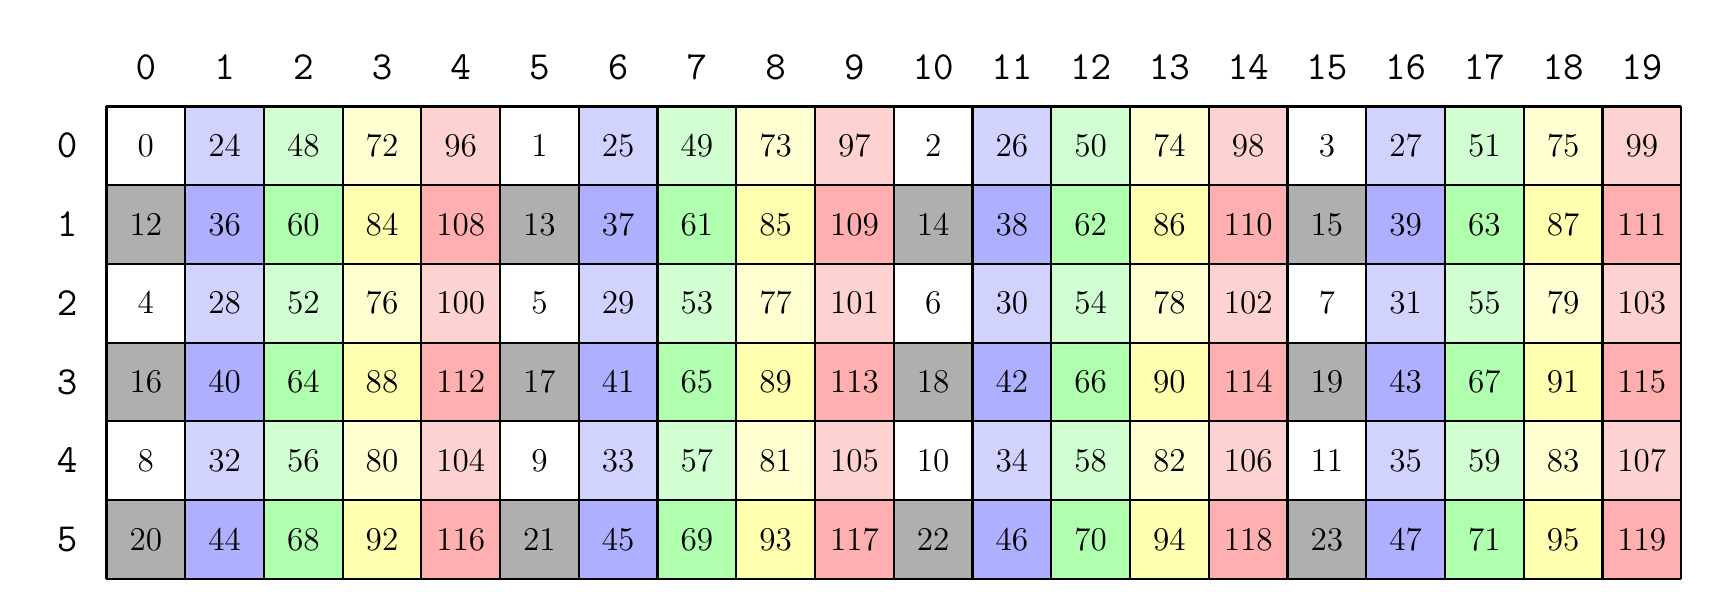
\begin{tikzpicture}[x={(0cm,-1cm)},y={(1cm,0cm)},every node/.style={minimum size=1cm, outer sep=0pt}]

\node[fill={rgb,255:red,255;green,255;blue,255}] at (0,0) {\large 0};
\node[fill={rgb,255:red,210;green,210;blue,255}] at (0,1) {\large 24};
\node[fill={rgb,255:red,210;green,255;blue,210}] at (0,2) {\large 48};
\node[fill={rgb,255:red,255;green,255;blue,210}] at (0,3) {\large 72};
\node[fill={rgb,255:red,255;green,210;blue,210}] at (0,4) {\large 96};
\node[fill={rgb,255:red,255;green,255;blue,255}] at (0,5) {\large 1};
\node[fill={rgb,255:red,210;green,210;blue,255}] at (0,6) {\large 25};
\node[fill={rgb,255:red,210;green,255;blue,210}] at (0,7) {\large 49};
\node[fill={rgb,255:red,255;green,255;blue,210}] at (0,8) {\large 73};
\node[fill={rgb,255:red,255;green,210;blue,210}] at (0,9) {\large 97};
\node[fill={rgb,255:red,255;green,255;blue,255}] at (0,10) {\large 2};
\node[fill={rgb,255:red,210;green,210;blue,255}] at (0,11) {\large 26};
\node[fill={rgb,255:red,210;green,255;blue,210}] at (0,12) {\large 50};
\node[fill={rgb,255:red,255;green,255;blue,210}] at (0,13) {\large 74};
\node[fill={rgb,255:red,255;green,210;blue,210}] at (0,14) {\large 98};
\node[fill={rgb,255:red,255;green,255;blue,255}] at (0,15) {\large 3};
\node[fill={rgb,255:red,210;green,210;blue,255}] at (0,16) {\large 27};
\node[fill={rgb,255:red,210;green,255;blue,210}] at (0,17) {\large 51};
\node[fill={rgb,255:red,255;green,255;blue,210}] at (0,18) {\large 75};
\node[fill={rgb,255:red,255;green,210;blue,210}] at (0,19) {\large 99};
\node[fill={rgb,255:red,175;green,175;blue,175}] at (1,0) {\large 12};
\node[fill={rgb,255:red,175;green,175;blue,255}] at (1,1) {\large 36};
\node[fill={rgb,255:red,175;green,255;blue,175}] at (1,2) {\large 60};
\node[fill={rgb,255:red,255;green,255;blue,175}] at (1,3) {\large 84};
\node[fill={rgb,255:red,255;green,175;blue,175}] at (1,4) {\large 108};
\node[fill={rgb,255:red,175;green,175;blue,175}] at (1,5) {\large 13};
\node[fill={rgb,255:red,175;green,175;blue,255}] at (1,6) {\large 37};
\node[fill={rgb,255:red,175;green,255;blue,175}] at (1,7) {\large 61};
\node[fill={rgb,255:red,255;green,255;blue,175}] at (1,8) {\large 85};
\node[fill={rgb,255:red,255;green,175;blue,175}] at (1,9) {\large 109};
\node[fill={rgb,255:red,175;green,175;blue,175}] at (1,10) {\large 14};
\node[fill={rgb,255:red,175;green,175;blue,255}] at (1,11) {\large 38};
\node[fill={rgb,255:red,175;green,255;blue,175}] at (1,12) {\large 62};
\node[fill={rgb,255:red,255;green,255;blue,175}] at (1,13) {\large 86};
\node[fill={rgb,255:red,255;green,175;blue,175}] at (1,14) {\large 110};
\node[fill={rgb,255:red,175;green,175;blue,175}] at (1,15) {\large 15};
\node[fill={rgb,255:red,175;green,175;blue,255}] at (1,16) {\large 39};
\node[fill={rgb,255:red,175;green,255;blue,175}] at (1,17) {\large 63};
\node[fill={rgb,255:red,255;green,255;blue,175}] at (1,18) {\large 87};
\node[fill={rgb,255:red,255;green,175;blue,175}] at (1,19) {\large 111};
\node[fill={rgb,255:red,255;green,255;blue,255}] at (2,0) {\large 4};
\node[fill={rgb,255:red,210;green,210;blue,255}] at (2,1) {\large 28};
\node[fill={rgb,255:red,210;green,255;blue,210}] at (2,2) {\large 52};
\node[fill={rgb,255:red,255;green,255;blue,210}] at (2,3) {\large 76};
\node[fill={rgb,255:red,255;green,210;blue,210}] at (2,4) {\large 100};
\node[fill={rgb,255:red,255;green,255;blue,255}] at (2,5) {\large 5};
\node[fill={rgb,255:red,210;green,210;blue,255}] at (2,6) {\large 29};
\node[fill={rgb,255:red,210;green,255;blue,210}] at (2,7) {\large 53};
\node[fill={rgb,255:red,255;green,255;blue,210}] at (2,8) {\large 77};
\node[fill={rgb,255:red,255;green,210;blue,210}] at (2,9) {\large 101};
\node[fill={rgb,255:red,255;green,255;blue,255}] at (2,10) {\large 6};
\node[fill={rgb,255:red,210;green,210;blue,255}] at (2,11) {\large 30};
\node[fill={rgb,255:red,210;green,255;blue,210}] at (2,12) {\large 54};
\node[fill={rgb,255:red,255;green,255;blue,210}] at (2,13) {\large 78};
\node[fill={rgb,255:red,255;green,210;blue,210}] at (2,14) {\large 102};
\node[fill={rgb,255:red,255;green,255;blue,255}] at (2,15) {\large 7};
\node[fill={rgb,255:red,210;green,210;blue,255}] at (2,16) {\large 31};
\node[fill={rgb,255:red,210;green,255;blue,210}] at (2,17) {\large 55};
\node[fill={rgb,255:red,255;green,255;blue,210}] at (2,18) {\large 79};
\node[fill={rgb,255:red,255;green,210;blue,210}] at (2,19) {\large 103};
\node[fill={rgb,255:red,175;green,175;blue,175}] at (3,0) {\large 16};
\node[fill={rgb,255:red,175;green,175;blue,255}] at (3,1) {\large 40};
\node[fill={rgb,255:red,175;green,255;blue,175}] at (3,2) {\large 64};
\node[fill={rgb,255:red,255;green,255;blue,175}] at (3,3) {\large 88};
\node[fill={rgb,255:red,255;green,175;blue,175}] at (3,4) {\large 112};
\node[fill={rgb,255:red,175;green,175;blue,175}] at (3,5) {\large 17};
\node[fill={rgb,255:red,175;green,175;blue,255}] at (3,6) {\large 41};
\node[fill={rgb,255:red,175;green,255;blue,175}] at (3,7) {\large 65};
\node[fill={rgb,255:red,255;green,255;blue,175}] at (3,8) {\large 89};
\node[fill={rgb,255:red,255;green,175;blue,175}] at (3,9) {\large 113};
\node[fill={rgb,255:red,175;green,175;blue,175}] at (3,10) {\large 18};
\node[fill={rgb,255:red,175;green,175;blue,255}] at (3,11) {\large 42};
\node[fill={rgb,255:red,175;green,255;blue,175}] at (3,12) {\large 66};
\node[fill={rgb,255:red,255;green,255;blue,175}] at (3,13) {\large 90};
\node[fill={rgb,255:red,255;green,175;blue,175}] at (3,14) {\large 114};
\node[fill={rgb,255:red,175;green,175;blue,175}] at (3,15) {\large 19};
\node[fill={rgb,255:red,175;green,175;blue,255}] at (3,16) {\large 43};
\node[fill={rgb,255:red,175;green,255;blue,175}] at (3,17) {\large 67};
\node[fill={rgb,255:red,255;green,255;blue,175}] at (3,18) {\large 91};
\node[fill={rgb,255:red,255;green,175;blue,175}] at (3,19) {\large 115};
\node[fill={rgb,255:red,255;green,255;blue,255}] at (4,0) {\large 8};
\node[fill={rgb,255:red,210;green,210;blue,255}] at (4,1) {\large 32};
\node[fill={rgb,255:red,210;green,255;blue,210}] at (4,2) {\large 56};
\node[fill={rgb,255:red,255;green,255;blue,210}] at (4,3) {\large 80};
\node[fill={rgb,255:red,255;green,210;blue,210}] at (4,4) {\large 104};
\node[fill={rgb,255:red,255;green,255;blue,255}] at (4,5) {\large 9};
\node[fill={rgb,255:red,210;green,210;blue,255}] at (4,6) {\large 33};
\node[fill={rgb,255:red,210;green,255;blue,210}] at (4,7) {\large 57};
\node[fill={rgb,255:red,255;green,255;blue,210}] at (4,8) {\large 81};
\node[fill={rgb,255:red,255;green,210;blue,210}] at (4,9) {\large 105};
\node[fill={rgb,255:red,255;green,255;blue,255}] at (4,10) {\large 10};
\node[fill={rgb,255:red,210;green,210;blue,255}] at (4,11) {\large 34};
\node[fill={rgb,255:red,210;green,255;blue,210}] at (4,12) {\large 58};
\node[fill={rgb,255:red,255;green,255;blue,210}] at (4,13) {\large 82};
\node[fill={rgb,255:red,255;green,210;blue,210}] at (4,14) {\large 106};
\node[fill={rgb,255:red,255;green,255;blue,255}] at (4,15) {\large 11};
\node[fill={rgb,255:red,210;green,210;blue,255}] at (4,16) {\large 35};
\node[fill={rgb,255:red,210;green,255;blue,210}] at (4,17) {\large 59};
\node[fill={rgb,255:red,255;green,255;blue,210}] at (4,18) {\large 83};
\node[fill={rgb,255:red,255;green,210;blue,210}] at (4,19) {\large 107};
\node[fill={rgb,255:red,175;green,175;blue,175}] at (5,0) {\large 20};
\node[fill={rgb,255:red,175;green,175;blue,255}] at (5,1) {\large 44};
\node[fill={rgb,255:red,175;green,255;blue,175}] at (5,2) {\large 68};
\node[fill={rgb,255:red,255;green,255;blue,175}] at (5,3) {\large 92};
\node[fill={rgb,255:red,255;green,175;blue,175}] at (5,4) {\large 116};
\node[fill={rgb,255:red,175;green,175;blue,175}] at (5,5) {\large 21};
\node[fill={rgb,255:red,175;green,175;blue,255}] at (5,6) {\large 45};
\node[fill={rgb,255:red,175;green,255;blue,175}] at (5,7) {\large 69};
\node[fill={rgb,255:red,255;green,255;blue,175}] at (5,8) {\large 93};
\node[fill={rgb,255:red,255;green,175;blue,175}] at (5,9) {\large 117};
\node[fill={rgb,255:red,175;green,175;blue,175}] at (5,10) {\large 22};
\node[fill={rgb,255:red,175;green,175;blue,255}] at (5,11) {\large 46};
\node[fill={rgb,255:red,175;green,255;blue,175}] at (5,12) {\large 70};
\node[fill={rgb,255:red,255;green,255;blue,175}] at (5,13) {\large 94};
\node[fill={rgb,255:red,255;green,175;blue,175}] at (5,14) {\large 118};
\node[fill={rgb,255:red,175;green,175;blue,175}] at (5,15) {\large 23};
\node[fill={rgb,255:red,175;green,175;blue,255}] at (5,16) {\large 47};
\node[fill={rgb,255:red,175;green,255;blue,175}] at (5,17) {\large 71};
\node[fill={rgb,255:red,255;green,255;blue,175}] at (5,18) {\large 95};
\node[fill={rgb,255:red,255;green,175;blue,175}] at (5,19) {\large 119};
\draw[color=black,thick,shift={(-0.5,-0.5)}] (0,0) grid (6,20);

\node at (0,-1) {\Large{\texttt{0}}};
\node at (1,-1) {\Large{\texttt{1}}};
\node at (2,-1) {\Large{\texttt{2}}};
\node at (3,-1) {\Large{\texttt{3}}};
\node at (4,-1) {\Large{\texttt{4}}};
\node at (5,-1) {\Large{\texttt{5}}};
\node at (-1,0) {\Large{\texttt{0}}};
\node at (-1,1) {\Large{\texttt{1}}};
\node at (-1,2) {\Large{\texttt{2}}};
\node at (-1,3) {\Large{\texttt{3}}};
\node at (-1,4) {\Large{\texttt{4}}};
\node at (-1,5) {\Large{\texttt{5}}};
\node at (-1,6) {\Large{\texttt{6}}};
\node at (-1,7) {\Large{\texttt{7}}};
\node at (-1,8) {\Large{\texttt{8}}};
\node at (-1,9) {\Large{\texttt{9}}};
\node at (-1,10) {\Large{\texttt{10}}};
\node at (-1,11) {\Large{\texttt{11}}};
\node at (-1,12) {\Large{\texttt{12}}};
\node at (-1,13) {\Large{\texttt{13}}};
\node at (-1,14) {\Large{\texttt{14}}};
\node at (-1,15) {\Large{\texttt{15}}};
\node at (-1,16) {\Large{\texttt{16}}};
\node at (-1,17) {\Large{\texttt{17}}};
\node at (-1,18) {\Large{\texttt{18}}};
\node at (-1,19) {\Large{\texttt{19}}};
\end{tikzpicture}
}
\caption{行主序 $(3,4):(4,1)$ 瓦片与列主序 $(2,5):(1,2)$ 铺瓦的 {\tt raked\_product}。}
\label{fig:rakedproduct}
\end{figure}

%The operation {\tt tiled\_product} is another convenience function that simply flattens by one level the second mode of a logical product.

还可以构造逻辑乘积的许多其它版本，它们额外地对模进行分组与重排，以得到方便使用的结果。

\wpssh{应用：逻辑切分}
\label{sec:logical_divide}

两个布局 $\v{A}$ 与 $\v{B}$ 的逻辑切分是一个布局 $\v{R}$，其中“布局 $\v{A}$ 被一分为二：被 $\v{B}$ 指向的元素与未被 $\v{B}$ 指向的元素”。

具体地，我们将逻辑切分定义为一个从两个布局产生一个 2 阶布局的函数
\begin{align*}
\v{A} \oslash \v{B} = \v{A} \circ (\v{B}, \v{B}^*_{\abs{\v{A}}}) = \v{A} \circ \v{B}^\bigstar
\end{align*}
其中 $\v{B}^*_{\abs{\v{A}}}$ 是 $\v{B}$ 相对于布局 $\v{A}$ 的尺寸所取的补。由于该操作意在保留 $\v{A}$ 的全部元素、只是把布局 $\v{A}$ 一分为二，我们要求 $\v{B}^\bigstar = (\v{B},\v{B}^*_{\abs{\v{A}}})$ 满射到 $\Z_{\abs{A}}$。这通常涉及对 $\v{B}^*$ 尺寸的扩展，使得 $\abs{\v{B}^\bigstar} \geq \abs{\v{A}}$。此外，我们要求补 $\v{B}^*$ 在如下意义上“补全”布局 $\v{B}$：$\v{B}^\bigstar = (\v{B},\v{B}^*_{\abs{A}})$ 具有自反广义逆 $\v{B}^+$，满足
\begin{align}
\v{B}^\bigstar \v{B}^+ \v{B}^\bigstar = \v{B}^\bigstar \\
\v{B}^+ \v{B}^\bigstar \v{B}^+ = \v{B}^+
\end{align}

与逻辑乘积操作类似，结果布局 $\v{A} \circ \v{B}$ 的第一个模通常被称为“瓦片”，它在“网格”（即“铺瓦”）布局 $\v{A} \circ \v{B}^*_{\abs{\v{A}}}$ 上被重复。参数 $\v{B}$ 被称为“铺瓦器”，它可以被扩展为不仅仅是布局，如第~\ref{sec:tiler}~节所述。

作为一个直接的例子，常见的需求是从另一个布局中取出某组逻辑元素。例如，要从布局中每隔三个取一个元素，可以使用复合：
\begin{align*}
\begin{array}{c} \textcolor{red}{24} \\ \textcolor{red}{3} \end{array}
\ \circ \
\begin{array}{c} \textcolor{blue}{8} \\ \textcolor{blue}{3} \end{array}
\ &= \
\begin{array}{c} \textcolor{blue}{8} \\ \textcolor{blue}{9} \end{array} \\
\begin{array}{ccc} (\textcolor{red}{6}, & \textcolor{red}{2}, & \textcolor{red}{2}) \\ (\textcolor{red}{2}, & \textcolor{red}{1}, & \textcolor{red}{20}) \end{array}
\ \circ \
\begin{array}{c} \textcolor{blue}{8} \\ \textcolor{blue}{3} \end{array}
\ &= \
\begin{array}{ccc} (\textcolor{blue}{2}, & \textcolor{blue}{2}, & \textcolor{blue}{2}) \\ (\textcolor{blue}{6}, & \textcolor{blue}{1}, & \textcolor{blue}{20}) \end{array}
\end{align*}
在上面两种情形中，都是 24 个元素的布局与布局 $8:3$ 复合，得到每隔三个取一个元素的布局。但左手边布局中“其余”的元素怎么办？逻辑切分把左手边的布局拆成两块：被右手边“命中”的部分与“其余”部分：
\begin{align*}
\begin{array}{c} \textcolor{red}{24} \\ \textcolor{red}{3} \end{array}
\ \oslash \
\begin{array}{c} \textcolor{blue}{8} \\ \textcolor{blue}{3} \end{array}
\ &=& \
\begin{array}{c} \textcolor{red}{24} \\ \textcolor{red}{3} \end{array}
\ \circ \
\begin{array}{cc} (\textcolor{blue}{8}, & 3) \\ (\textcolor{blue}{3}, & 1) \end{array}
\ &=& \
\begin{array}{cc} (\textcolor{blue}{8}, & 3) \\ (\textcolor{blue}{9}, & 3) \end{array} \\
\begin{array}{ccc} (\textcolor{red}{6}, & \textcolor{red}{2}, & \textcolor{red}{2}) \\ (\textcolor{red}{2}, & \textcolor{red}{1}, & \textcolor{red}{20}) \end{array}
\ \oslash \
\begin{array}{c} \textcolor{blue}{8} \\ \textcolor{blue}{3} \end{array}
\ &=& \
\begin{array}{ccc} (\textcolor{red}{6}, & \textcolor{red}{2}, & \textcolor{red}{2}) \\ (\textcolor{red}{2}, & \textcolor{red}{1}, & \textcolor{red}{20}) \end{array}
\ \circ \
\begin{array}{cc} (\textcolor{blue}{8}, & 3) \\ (\textcolor{blue}{3}, & 1) \end{array}
\ &=& \
\begin{array}{cccc} ((\textcolor{blue}{2}, & \textcolor{blue}{2}, & \textcolor{blue}{2}), & 3) \\ ((\textcolor{blue}{6}, & \textcolor{blue}{1}, & \textcolor{blue}{20}), & 2) \end{array}
\end{align*}
其中 $3:1$ 是 $8:3$ 在尺寸 24 之下的补。结果的第一模按要求仍然包含左手边布局中每隔三个取一个的元素，而结果的第二模是这些“瓦片”在原布局中的个数（本例中为 3）以及这些瓦片之间的步幅。补被用来确定缺失了哪些元素、以及以何种顺序保留它们。

\paragraph{相关切分}

与复合类似，人们经常希望按模施加逻辑切分。这里使用同样的记号与策略
\begin{align*}
\v{A} \oslash \langle \v{B},\v{C} \rangle = (\v{A}_0,\v{A}_1) \oslash \langle \v{B},\v{C} \rangle = (\v{A}_0 \oslash \v{B}, \v{A}_1 \oslash \v{C}).
\end{align*}
其直觉在于：能够对列和行独立地执行这些操作，然后视需要重排这些模以构造新布局，这与布局乘积类似。例如，回到第~\ref{sec:tiler}~节中的铺瓦器，将这些铺瓦器用于逻辑切分而非复合，就得到铺瓦器所指向的 $4 {\times} 8$ 子布局组成的 $2 {\times} 2$ 布局。图~\ref{fig:tilers_divide} 展示了这一点，其中可以想象有一个 $2 {\times} 2$ 布局映射到每个单独施以底纹的数据瓦片。

\begin{figure}[ht]
\centering
\begin{subfigure}{0.22\textwidth}
\centering
\resizebox{\linewidth}{!}{
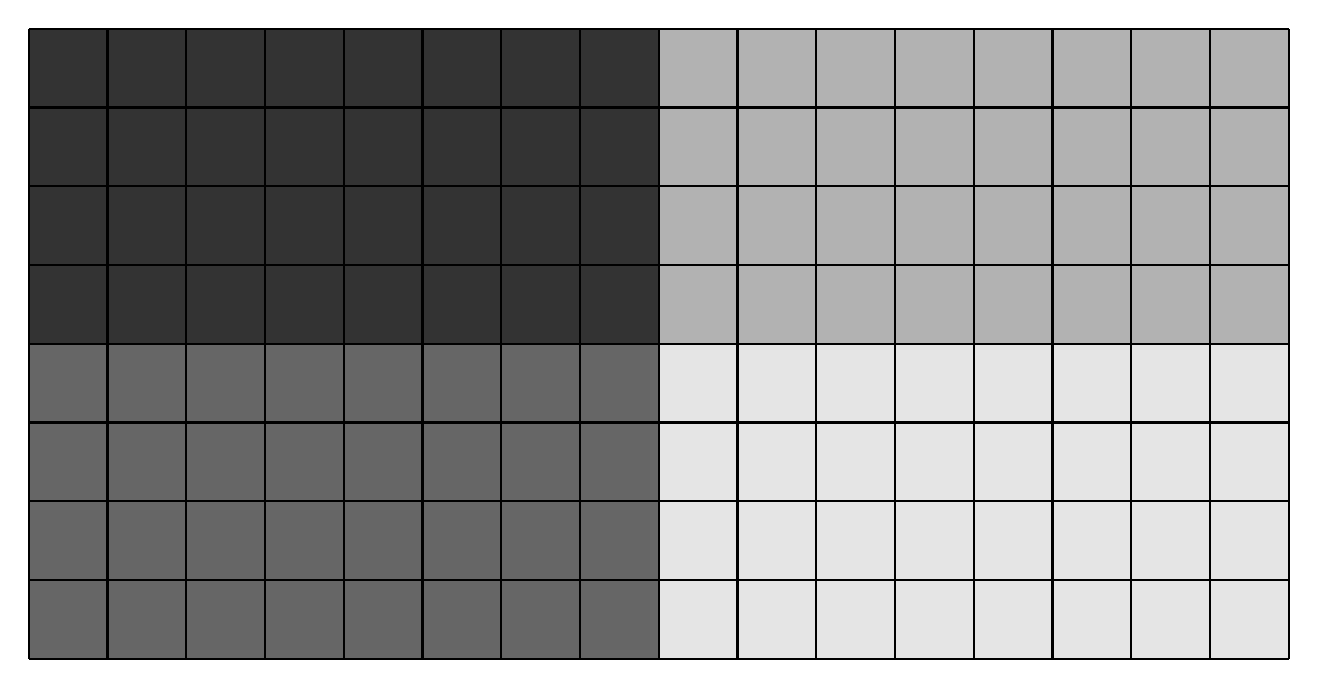
\begin{tikzpicture}[x={(0cm,-1cm)},y={(1cm,0cm)},every node/.style={minimum size=1cm, outer sep=0pt}]
\foreach \i in {0,1,2,3} {
\foreach \j in {0,1,2,3,4,5,6,7} {
\node[fill=black!80!white] at (\i,\j) {};
}}
\foreach \i in {4,5,6,7} {
\foreach \j in {0,1,2,3,4,5,6,7} {
\node[fill=black!60!white] at (\i,\j) {};
}}
\foreach \i in {0,1,2,3} {
\foreach \j in {8,9,10,11,12,13,14,15} {
\node[fill=black!30!white] at (\i,\j) {};
}}
\foreach \i in {4,5,6,7} {
\foreach \j in {8,9,10,11,12,13,14,15} {
\node[fill=black!10!white] at (\i,\j) {};
}}
\draw[color=black,thick,shift={(-0.5,-0.5)}] (0,0) grid (8,16);
\end{tikzpicture}}
\caption{$\langle 4,8 \rangle \equiv \langle 4:1,8:1 \rangle$}
\end{subfigure}\quad
\begin{subfigure}{0.22\textwidth}
\centering
\resizebox{\linewidth}{!}{
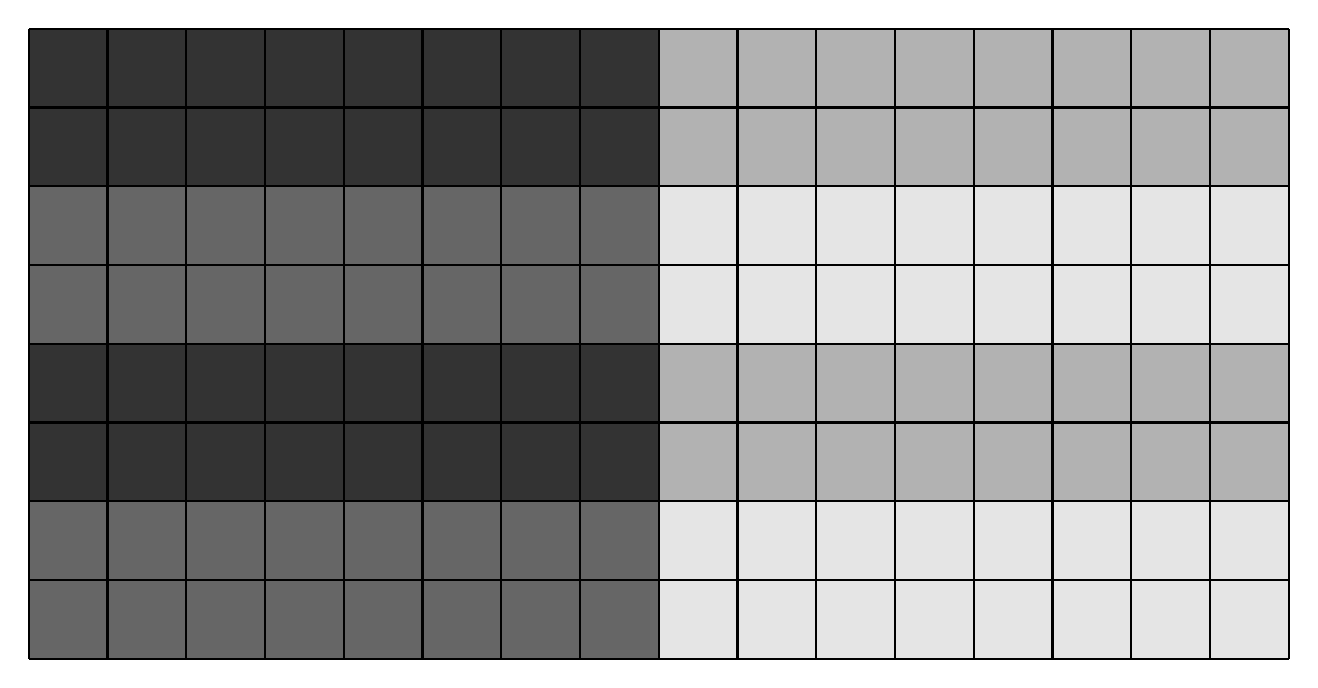
\begin{tikzpicture}[x={(0cm,-1cm)},y={(1cm,0cm)},every node/.style={minimum size=1cm, outer sep=0pt}]
\foreach \i in {0,1,4,5} {
\foreach \j in {0,1,2,3,4,5,6,7} {
\node[fill=black!80!white] at (\i,\j) {};
}}
\foreach \i in {2,3,6,7} {
\foreach \j in {0,1,2,3,4,5,6,7} {
\node[fill=black!60!white] at (\i,\j) {};
}}
\foreach \i in {0,1,4,5} {
\foreach \j in {8,9,10,11,12,13,14,15} {
\node[fill=black!30!white] at (\i,\j) {};
}}
\foreach \i in {2,3,6,7} {
\foreach \j in {8,9,10,11,12,13,14,15} {
\node[fill=black!10!white] at (\i,\j) {};
}}
\draw[color=black,thick,shift={(-0.5,-0.5)}] (0,0) grid (8,16);
\end{tikzpicture}}
\caption{$\langle (2,2):(1,4),8:1 \rangle$}
\end{subfigure}\quad
\begin{subfigure}{0.22\textwidth}
\centering
\resizebox{\linewidth}{!}{
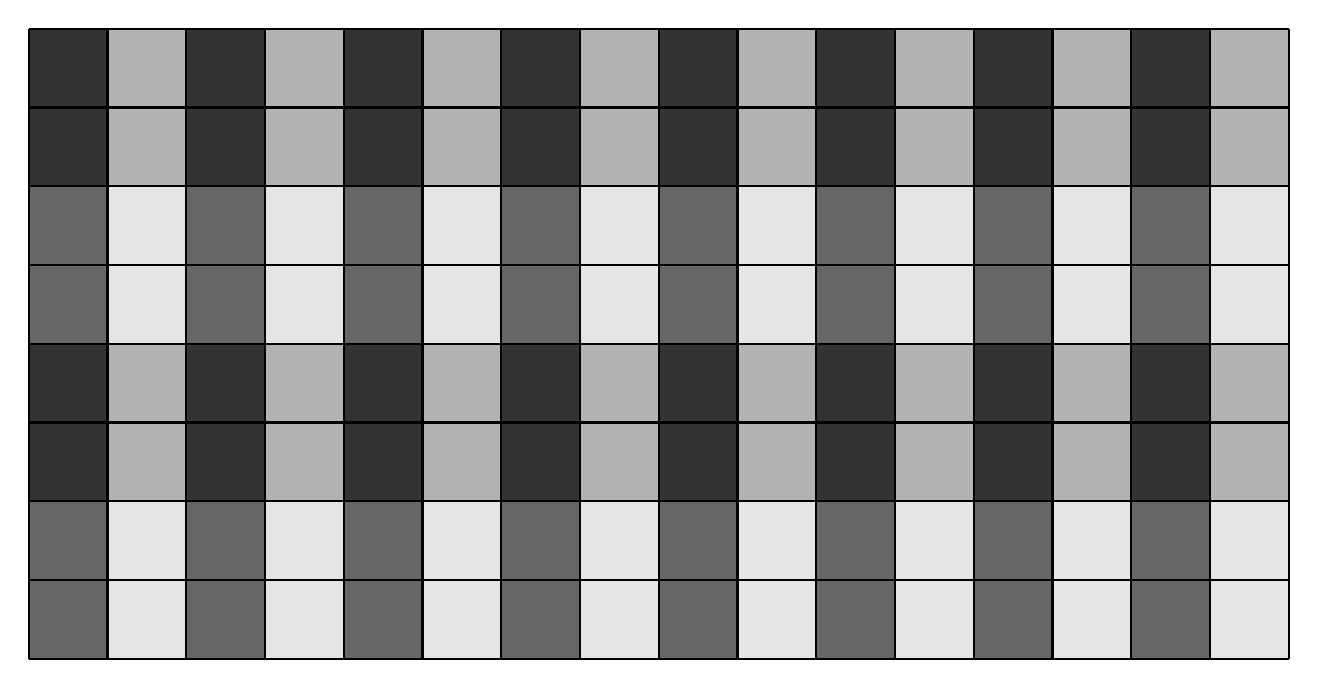
\begin{tikzpicture}[x={(0cm,-1cm)},y={(1cm,0cm)},every node/.style={minimum size=1cm, outer sep=0pt}]
\foreach \i in {0,1,4,5} {
\foreach \j in {0,2,4,6,8,10,12,14} {
\node[fill=black!80!white] at (\i,\j) {};
}}
\foreach \i in {2,3,6,7} {
\foreach \j in {0,2,4,6,8,10,12,14} {
\node[fill=black!60!white] at (\i,\j) {};
}}
\foreach \i in {0,1,4,5} {
\foreach \j in {1,3,5,7,9,11,13,15} {
\node[fill=black!30!white] at (\i,\j) {};
}}
\foreach \i in {2,3,6,7} {
\foreach \j in {1,3,5,7,9,11,13,15} {
\node[fill=black!10!white] at (\i,\j) {};
}}
\draw[color=black,thick,shift={(-0.5,-0.5)}] (0,0) grid (8,16);
\end{tikzpicture}}
\caption{$\langle (2,2):(1,4),8:2 \rangle$}
\end{subfigure}\quad
\begin{subfigure}{0.22\textwidth}
\centering
\resizebox{\linewidth}{!}{
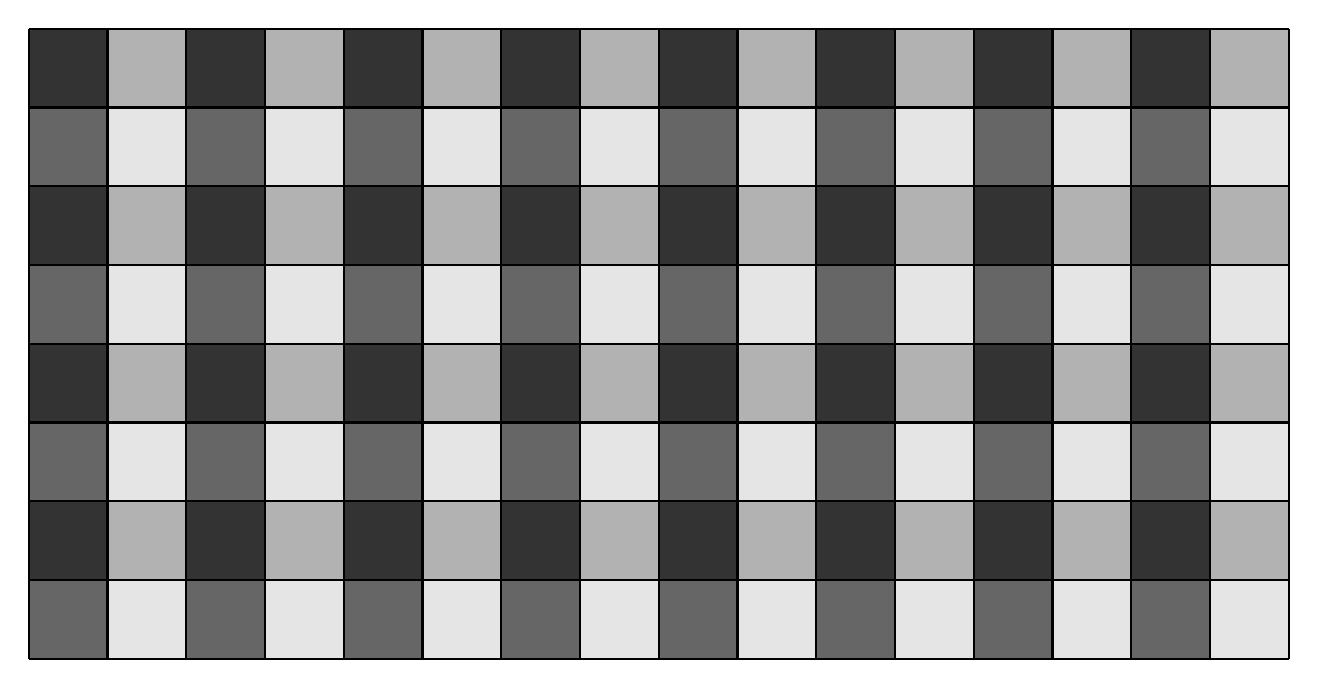
\begin{tikzpicture}[x={(0cm,-1cm)},y={(1cm,0cm)},every node/.style={minimum size=1cm, outer sep=0pt}]
\foreach \i in {0,2,4,6} {
\foreach \j in {0,2,4,6,8,10,12,14} {
\node[fill=black!80!white] at (\i,\j) {};
}}
\foreach \i in {1,3,5,7} {
\foreach \j in {0,2,4,6,8,10,12,14} {
\node[fill=black!60!white] at (\i,\j) {};
}}
\foreach \i in {0,2,4,6} {
\foreach \j in {1,3,5,7,9,11,13,15} {
\node[fill=black!30!white] at (\i,\j) {};
}}
\foreach \i in {1,3,5,7} {
\foreach \j in {1,3,5,7,9,11,13,15} {
\node[fill=black!10!white] at (\i,\j) {};
}}
\draw[color=black,thick,shift={(-0.5,-0.5)}] (0,0) grid (8,16);
\end{tikzpicture}}
\caption{$\langle 4:2,8:2 \rangle$}
\end{subfigure}
\caption{将 $8 {\times} 16$ 布局切分为 $4 {\times} 8$ 瓦片、并以 $2 {\times} 2$ 铺瓦的铺瓦器示例。}
\label{fig:tilers_divide}
\end{figure}

例如，给定布局 $(\textcolor{red}{8},\textcolor{red}{16}):(\textcolor{red}{20},\textcolor{red}{1})$，我们想抽取一个“瓦片”：沿每列向下取 4 个连续元素、沿每行每隔一个取一个元素。按模的逻辑切分给出
\begin{align*}
\begin{array}{cc} (\textcolor{red}{8}, & \textcolor{red}{16})\\
                  (\textcolor{red}{20},& \textcolor{red}{1}) \end{array}
\ \oslash \
\left\langle
\begin{array}{c} \textcolor{blue}{4} \\ \textcolor{blue}{1} \end{array},
\begin{array}{c} \textcolor{blue}{8} \\ \textcolor{blue}{2} \end{array}
\right\rangle
\ = \
\begin{array}{cc} (\textcolor{red}{8}, & \textcolor{red}{16}) \\ (\textcolor{red}{20}, & \textcolor{red}{1}) \end{array}
\ \circ \
\left\langle
\begin{array}{cc} (\textcolor{blue}{4}, & \textcolor{black}{2}) \\ (\textcolor{blue}{1}, & \textcolor{black}{4}) \end{array},
\begin{array}{cc} (\textcolor{blue}{8}, & \textcolor{black}{2}) \\ (\textcolor{blue}{2}, & \textcolor{black}{1}) \end{array}
\right\rangle
\ = \
\begin{array}{cccc}((\textcolor{blue}{4}, & \textcolor{black}{2}), & (\textcolor{blue}{8}, & \textcolor{black}{2})) \\ ((\textcolor{blue}{20}, & \textcolor{black}{80}), & (\textcolor{blue}{2}, & \textcolor{black}{1})) \end{array}
\end{align*}
其中“瓦片”模标为蓝色，“其余”模标为黑色。注意，结果布局仍保持 $8 {\times} 16$，而铺瓦器所指向的元素已被置换到最前面的 $4 {\times} 8$ 块中。

操作 {\tt zipped\_divide} 先执行按模逻辑切分，再把同类模拉链式地组合在一起：
\begin{align*}
\begin{array}{cccc}((\textcolor{blue}{4}, & \textcolor{blue}{8}), & (\textcolor{black}{2}, & \textcolor{black}{2})) \\ ((\textcolor{blue}{20}, & \textcolor{blue}{2}), & (\textcolor{black}{80}, & \textcolor{black}{1})) \end{array}
\end{align*}
这生成了一个“瓦片”模（蓝色），它恰好是铺瓦器所指向的子布局；以及一个“其余”模（黑色），它是遍历各瓦片的子布局。操作 {\tt zipped\_divide} 总是返回一个 2 阶布局结果，其第一模恰好是与铺瓦器的复合，第二模是与补的复合。

软件中一个非常常见的模式是：把数据布局铺瓦成一个瓦片网格，然后为每个处理单元选出特定的瓦片。在 Python 参考实现 PyCuTe（NVIDIA，2026）中，其形式如下：
\begin{python}
data    = Tensor(MyPtr, MyLayoutMxN)   # Tensor：Crd -> Offset
tiler   = (4,8)                        # Tiler：TileCoord -> Crd
data_vt = zipped_divide(data, tiler)   # Compose：(TileCrd,GridCrd) -> Offset
tile    = data_vt[:, blk_id]           # 按一维 block id 切片
tile    = data_vt[:, (blk_x, blk_y)]   # 按二维 block id 切片，二者等价
\end{python}
可以看出，这一模式与第~\ref{sec:layouttv}~节的线程-值分块非常相似，只不过这里真正指定的只有瓦片模，缺失的“网格”模作为铺瓦器的补被计算出来。这个形状为 $(\text{瓦片}, \text{网格})$ 的“补全”铺瓦器随后与数据复合，产生瓦片网格；再在第二模上按块标识符切片，即可为某个处理单元抽取特定的瓦片。

同样可以构造逻辑切分的许多其它版本，它们额外地对模进行分组与重排，以得到方便使用的结果。

\wph{结论}

本文提出了 \CuTe，一个用于表示与操纵张量布局的数学框架，以应对现代 GPU 架构日益增长的复杂性。凭借其分层布局表示，\CuTe 为编写与管理当代硬件上专用张量指令所需的复杂数据布局与分块（partition）模式提供了通用方法。凭借其丰富的代数运算，\CuTe 为高性能线性代数 kernel 开发中布局的操纵与新布局的生成提供了一条有原理依据的途径。二者结合，该表示与代数能够支持复杂的布局与分块、关注点分离，以及静态分析与优化。

\CuTe 布局表示的表达能力已在若干关键应用中被证明极具价值。\CuTe 便于将多种多样的算法——例如广义张量-张量收缩（GETT）与卷积（CONV）——表示为通用矩阵乘法（GEMM）的实例，从而促进代码复用与算法统一性。例如，\CuTe 允许矩阵无论其具体数据布局如何都用 $(m,n)$ 坐标（coordinate）索引，让通用算法与具体布局保持正交；同时，要求特定布局的算法或指令则能够静态地检查、验证并推演它们的张量参数。

\CuTe 布局代数使得张量布局的静态分析与变换成为可能，用以实现并验证通用算法。例如，它可以为 \texttt{COPY} 操作推导最大向量化机会，验证矩阵乘累加（\texttt{MMA}）与 \texttt{COPY} 指令的输入输出布局，并推导出最优的共享内存布局，包括避免 bank 冲突的 swizzle 模式。这些能力把布局管理从易错的手工过程转变为一种系统化、可验证的方法论。为支持对本文定义的学习、实验与验证，纯 Python 参考实现 PyCuTe（NVIDIA，2026）已在 \url{https://github.com/NVlabs/CuTe} 公开发布。

\CuTe 的实际影响体现在它成功部署于生产系统，最显著的是作为 NVIDIA CUTLASS v3 与 v4 库的基础。在 CUTLASS 以及 FlashAttention 等应用中的性能评估表明，\CuTe 的抽象不引入任何性能开销，同时显著加速了软件开发。该框架的采用验证了它的双重承诺：在保持手工优化代码性能特征的同时，大幅降低开发复杂度与开发时间。

展望未来，\CuTe 的数学基础与代数化方法使其成为一个能够持续适应未来架构创新的框架。通过将布局关注点与算法逻辑分离，并提供强大的编译期推理能力，\CuTe 确立了一种面向张量中心编程的方法论，能够满足各类计算系统与应用的需求。

\section*{致谢}
\addcontentsline{toc}{section}{致谢}

作者感谢 Vijay Thakkar 作为 \CuTe 的早期使用者，感谢他在 \CuTe 的普及及其与 CUTLASS 的集成中发挥的关键作用，以及他对 \CuTe 基础设计与部署的重要贡献。他还感谢 Andrew Kerr、Pradeep Ramani 与 Manish Gupta，感谢他们对于在 CUTLASS 中使用 \CuTe 的洞见，以及他们推动 \CuTe 在高性能 kernel 开发中的早期采用。他感谢 Muhammad Osama 与 Duane Merrill 在 \CuTe 原型上的早期实验工作，以及在最初 \CuTe 示例中所做的底层性能优化。最后，作者感谢 Michael Garland、Bastian Hagedorn、Jay Shah 与 Amanda Liu 提出的富有洞见的反馈，以及他们对 \CuTe 规范一次次提出的挑战与质询。
